\nopagebreak
\section{Theory}
\subsection{Plane parallel layer}
The investigated semiconductor samples can in first approximation be described as a plane parallel 
layer \ref{fig:fabry-perot} with a thickness $d$ and refractive index $N_2$ which acts like a fabry-perot interferometer.
\begin{figure}[h]
    \centering
    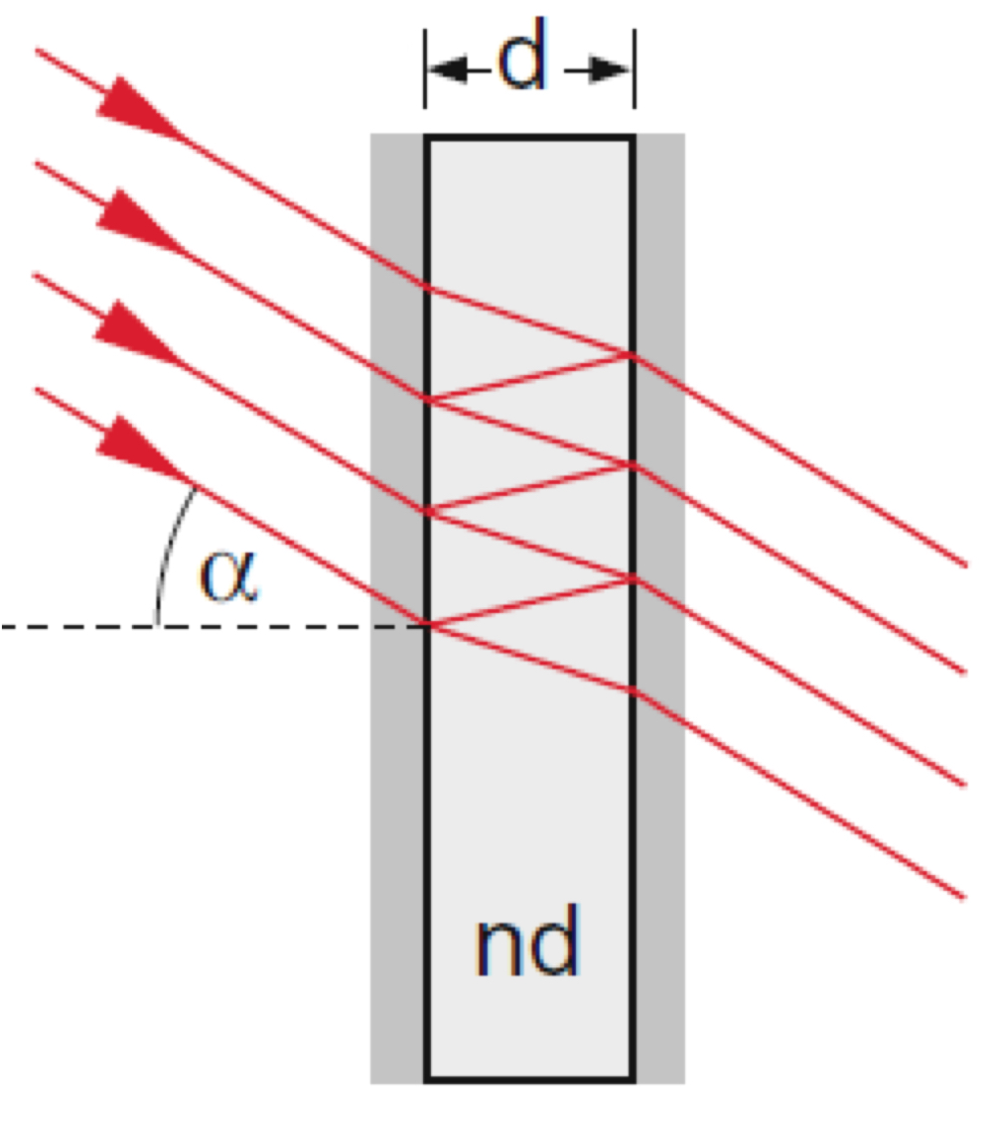
\includegraphics[width=0.3\textwidth]{Images/fabry-perot.png}
    \caption{Simplified illustration of the measured samples as a plane parallel plate
    with thickness $d$ and refractive index $N_2$. The surrounding air is described with a 
    refractive indes $N_1\approx1$ \cite{??}}
    \label{fig:fabry-perot}
\end{figure}
Light is simpliefied as beams. Every incoming beam is partially reflected and 
partially transmittet at the first interface. The total power reflectivity $R_1$ is described with:
\begin{align}
    R_1 = \left\lvert \frac{1 - N_2}{1 + N_2} \right\rvert^2 \label{eq:R1}
\end{align}
without considering the phase shift of the reflected beam. Like shown in the illustration, the total
power reflectivity of the second interface $R_2$ consists of the incoming beams and the beams reflected
at the first interface within the material. Additionally, the absorption of the material is considered.
Therefore, $R_2$ is described with:
\begin{align}
    R_2 = R_1(1-R_1)^2 \cdot e^{-2\beta d} \label{eq:R2}
\end{align}
with the absorption coefficient $\beta$ and the total power reflectivity $R_1$ of the first interface.
The assumption that the reflection of the first interface is the same as the reflection of the second
interface is in reality not correct. Disturbances like roughness of the interfaces or the absorption of the
material lead to a different reflection coeffitients of the two interfaces.\\
Considering this and the phase of the light, the total power reflectivity $R$ is described with:
\begin{align}
    R = \left\lvert \frac{(e^{i\frac{2\omega}{c}N_2d}-1)(1-N_2)}{e^{i\frac{2\omega}{c}N_2d}(1-N_2)-(1+N_2)} \right\rvert^2. \label{eq:R}
\end{align}
$\omega$ is the angular frequency of the light and $c$ the speed of light. 
The phase shift of the light is described with $e^{i\frac{2\omega}{c}N_2d}$. In contrast to \ref{eq:R2}, 
equation \ref{eq:R} shows a periodic modulation of the reflectivity because of interference.
The difference between the maxima of the modulation can be calculated with:
\begin{align}
    \Delta \nu = \nu_{\text{m+1}}-\nu_{\text{m}} = \frac{1}{2dN_2} \label{eq:delta_nu}
\end{align}
The refractive index $N_2$ can be calculated either with equation \ref{eq:delta_nu} or with
\begin{align}
    N_2 = \sqrt{\epsilon} \label{eq:nu}
\end{align}
using the square root of the dielectric function $\epsilon$ of the material.
The dielectric function $\epsilon$ is described in the drude model as:
\begin{align}
    \epsilon = 1-\frac{\omega^2_\text{p}\tau^2}{1+\omega^2\tau^2}+i\frac{\omega^2_\text{p}\tau}{\omega(1+\omega^2\tau^2)}
\end{align}
with $\omega_\text{p}$ as the plasma frequency:
\begin{align}
    \omega_\text{p} = \sqrt{\frac{N_\text{e}e^2}{\epsilon_0m^*}} \label{eq:omega_p}
\end{align}
and $\tau$ as the relaxation time of the electrons. 
$m^*$ is the effective mass of the electrons and $N_\text{e}$ the charge carrier density.
\\
For semiconductors, $\epsilon_\text{sem}$ can be calculated as:
\begin{align}
    \epsilon_\text{sem} = \epsilon_\text{LP} + i\frac{\sigma}{\omega\epsilon_0} \label{eq:epsilon_semiconductor}
\end{align}
with $\sigma$ as the conductivity of the semiconductor:
\begin{align}
    \sigma = \frac{N_\text{e}e^2\tau}{m^*}\frac{1}{1-i\omega\tau}. \label{eq:sigma}
\end{align}
The lattice contribution $\epsilon_\text{LP}$ is described as:
\begin{align}
    \epsilon_\text{LP} = \epsilon_\infty(1+\frac{\omega^2_\text{LO}-\omega^2_\text{TO}}{\omega^2_\text{TO}-\omega^2-i\Gamma\omega}) \label{eq:epsilon_LP}
\end{align}
with $\epsilon_\infty$ as the high frequency dielectric constant, $\omega_\text{LO}$ as the longitudinal optical phonon frequency,
$\omega_\text{TO}$ as the transversal optical phonon frequency and $\Gamma$ as the damping constant.
